\documentclass[12pt]{article}

\usepackage{amssymb,amsmath,amsthm}
\usepackage[top=1in, bottom=1in, left=1.25in, right=1.25in]{geometry}
\usepackage{fancyhdr}
\usepackage{enumerate}
\usepackage[bw,framed,numbered]{mcode}
\usepackage{graphicx}

% Comment the following line to use TeX's default font of Computer Modern.
\usepackage{times,txfonts}

\newtheoremstyle{homework}% name of the style to be used
  {18pt}% measure of space to leave above the theorem. E.g.: 3pt
  {12pt}% measure of space to leave below the theorem. E.g.: 3pt
  {}% name of font to use in the body of the theorem
  {}% measure of space to indent
  {\bfseries}% name of head font
  {:}% punctuation between head and body
  {2ex}% space after theorem head; " " = normal interword space
  {}% Manually specify head
\theoremstyle{homework} 

% Set up an Exercise environment and a Solution label.
\newtheorem*{exercisecore}{Exercise \@currentlabel}
\newenvironment{exercise}[1]
{\def\@currentlabel{#1}\exercisecore}
{\endexercisecore}

\newcommand{\localhead}[1]{\par\smallskip\noindent\textbf{#1}\nobreak\\}%
\newcommand\solution{\localhead{Solution:}}

%%%%%%%%%%%%%%%%%%%%%%%%%%%%%%%%%%%%%%%%%%%%%%%%%%%%%%%%%%%%%%%%%%%%%%%%
%
% Stuff for getting the name/document date/title across the header
\makeatletter
\RequirePackage{fancyhdr}
\pagestyle{fancy}
\fancyfoot[C]{\ifnum \value{page} > 1\relax\thepage\fi}
\fancyhead[L]{\ifx\@doclabel\@empty\else\@doclabel\fi}
\fancyhead[C]{\ifx\@docdate\@empty\else\@docdate\fi}
\fancyhead[R]{\ifx\@docauthor\@empty\else\@docauthor\fi}
\headheight 15pt

\def\doclabel#1{\gdef\@doclabel{#1}}
\doclabel{Use {\tt\textbackslash doclabel\{MY LABEL\}}.}
\def\docdate#1{\gdef\@docdate{#1}}
\docdate{Use {\tt\textbackslash docdate\{MY DATE\}}.}
\def\docauthor#1{\gdef\@docauthor{#1}}
\docauthor{Use {\tt\textbackslash docauthor\{MY NAME\}}.}
\makeatother

% Shortcuts for blackboard bold number sets (reals, integers, etc.)
\newcommand{\Reals}{\ensuremath{\mathbb R}}
\newcommand{\Nats}{\ensuremath{\mathbb N}}
\newcommand{\Ints}{\ensuremath{\mathbb Z}}
\newcommand{\Rats}{\ensuremath{\mathbb Q}}
\newcommand{\Cplx}{\ensuremath{\mathbb C}}
%% Some equivalents that some people may prefer.
\let\RR\Reals
\let\NN\Nats
\let\II\Ints
\let\CC\Cplx

%%%%%%%%%%%%%%%%%%%%%%%%%%%%%%%%%%%%%%%%%%%%%%%%%%%%%%%%%%%%%%%%%%%%%%%%%%%%%%%%%%%%%%%
%%%%%%%%%%%%%%%%%%%%%%%%%%%%%%%%%%%%%%%%%%%%%%%%%%%%%%%%%%%%%%%%%%%%%%%%%%%%%%%%%%%%%%%
% 
% The main document start here.

% The following commands set up the material that appears in the header.

%%%%%%%%%%%%%%%%%%%%%%%%%%%%%%%%%%%%%%%%%%%%%%%%%%%%%%%%%%%%%%%%%%%%%%%%%%%%%%%%%%%%%%%
%%%%%%%%%%%%%%%%%%%%%%%%%%%%%%%%%%%%%%%%%%%%%%%%%%%%%%%%%%%%%%%%%%%%%%%%%%%%%%%%%%%%%%%
% 
% The main document start here.

% The following commands set up the material that appears in the header.
\doclabel{STAT PHYS: Homework 3}
\docauthor{Parker Whaley}
\docdate{Feb 22, 2017}

\newcommand{\vv}{\mathbf{v}}
\begin{document}
\begin{exercise}{2.3}
\begin{enumerate}[(a)]
\item
There would be two possibilities for each coin so $2^{50}$ microstates.
\item
There are $\frac{50!}{25!}$ ways of choosing witch $25$ coins will be heads, however the order that we choose those coins in does not matter and so we need to eliminate the $25!$ overcounting and we see that there are $\frac{50!}{25!25!}$.
\item
$\frac{50!}{25!25!2^{50}}\approx 11.2\%$
\item
$\frac{50!}{30!20!2^{50}}\approx 4.1\%$
\item
$\frac{50!}{40!10!2^{50}}\approx 0.00091\%$
\item
$2^{-50}$
\item
in octave\\
\lstinputlisting{../octave/d1.txt}
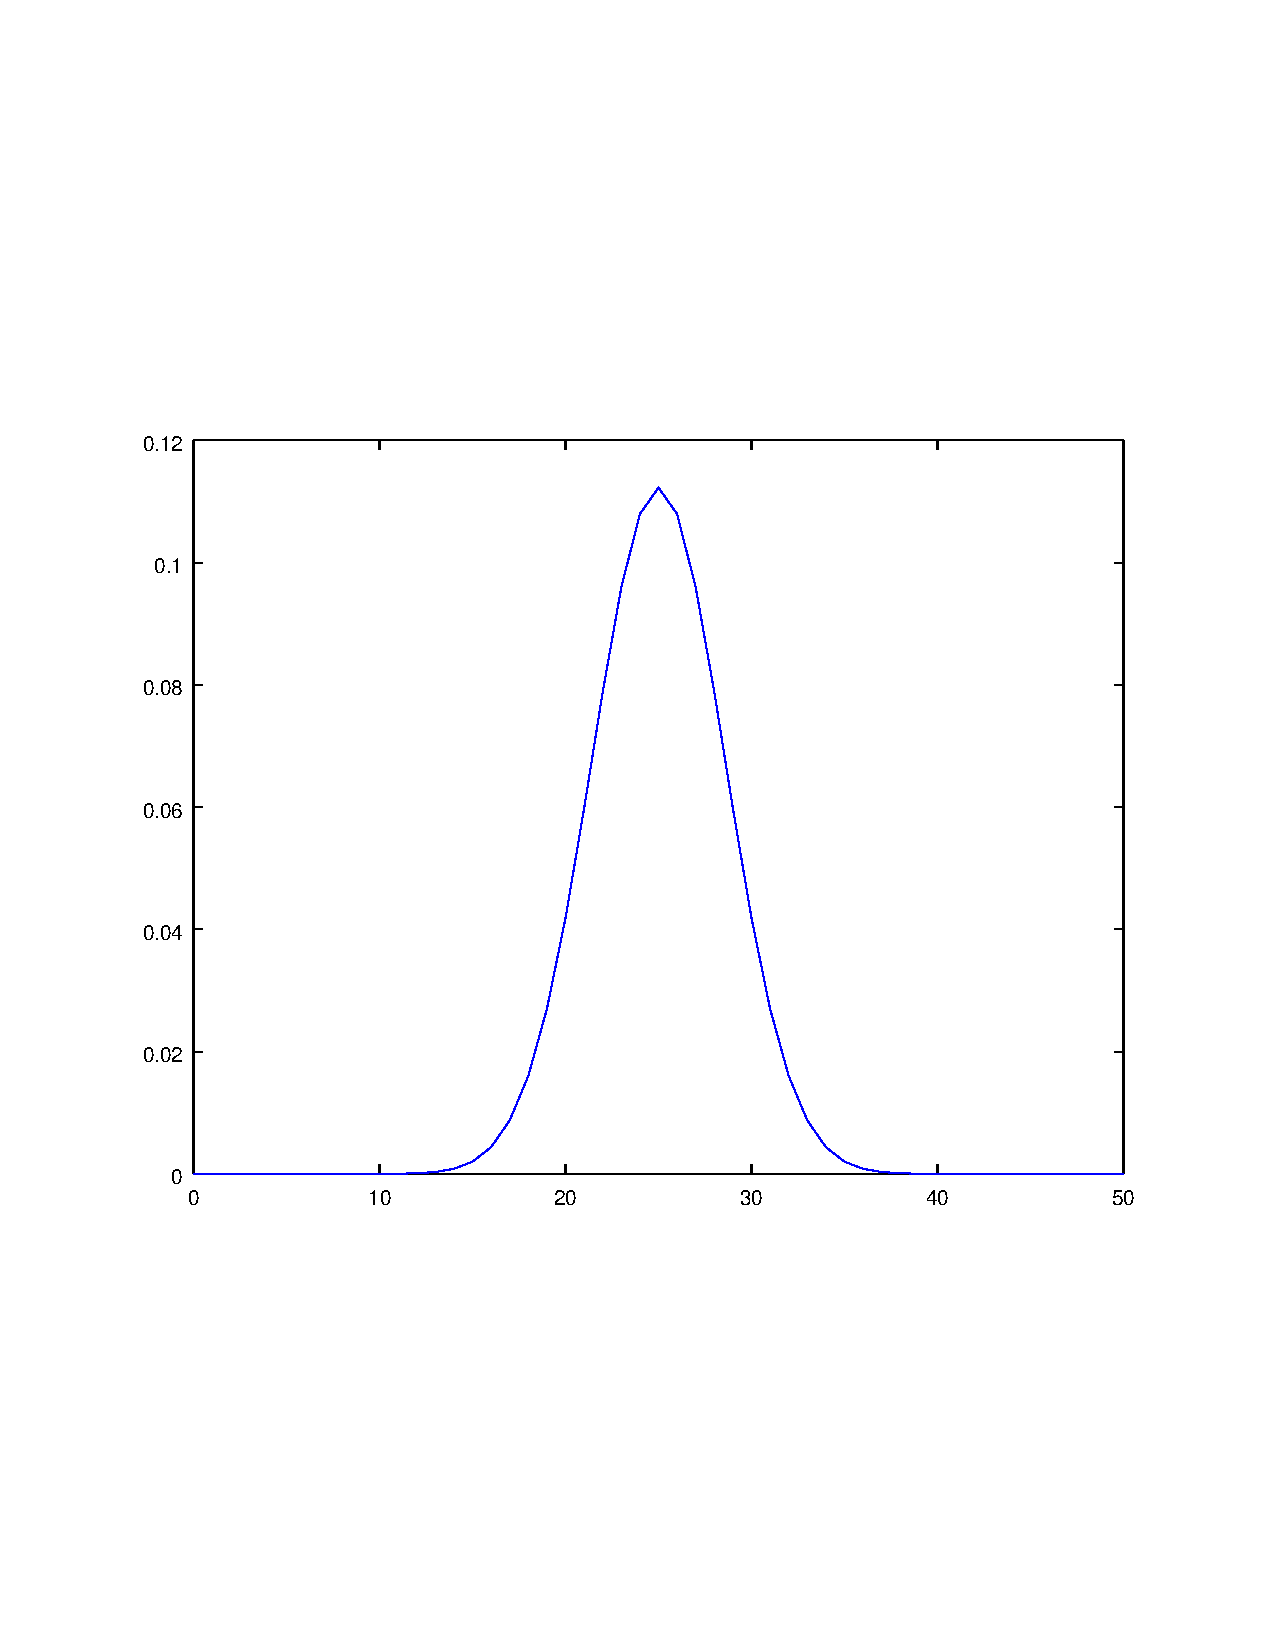
\includegraphics[scale=.35]{../octave/f1.pdf}

\end{enumerate}
\end{exercise}

\begin{exercise}{2.17}
$\ln(\Omega(N,q))\approx (q+N)\ln(q+N)-q\ln(q)-N\ln(N)$(2.18), Note that this equation is symetric under exchange of $N$ and $q$.  Thus since we already have a approximation when $q>>N$ we can by symetry simply swap $N$ and $q$ to obtain $\Omega(N,q)\approx e^{q\ln(N/q)}e^q=\biggr (\frac{eN}{q}\biggr)^q$ when $N>>q$.  Basically do all of the steps 2.19-2.21 with N and q exchanged and you get the previous result.
\end{exercise}

\begin{exercise}{2.18}
$\Omega(N,q)=\frac{(q+N-1)!}{q!(N-1)!}= \frac{N(q+N)!}{(q+N)q!N!}$, since $(A-1)!=\frac{A(A-1)!}{A}=\frac{A!}{A}$.  Applying Sterling's approximation of $A!=(A)^{A}e^{-A}\sqrt{2\pi A}$ we get $$\Omega(N,q)=\frac{N(q+N)!}{(q+N)q!N!}\approx\frac{N(q+N)^{q+N}e^{-(q+N)}\sqrt{2\pi (q+N)}}{(q+N)q^qe^{-q}\sqrt{2\pi q}N^Ne^{-N}\sqrt{2\pi N}}$$
$$=\frac{N(q+N)^{q+N}e^{-(q+N)}\sqrt{(q+N)}}{(q+N)q^qe^{-q}N^Ne^{-N}\sqrt{2\pi qN}}$$
$$=\frac{N(q+N)^{q+N}\sqrt{(q+N)}}{(q+N)q^qN^N\sqrt{2\pi qN}}$$
$$=\frac{N(q+N)^{q+N}}{\sqrt{(q+N)}q^qN^N\sqrt{2\pi qN}}$$
$$=\frac{(q+N)^{q+N}}{q^qN^N\sqrt{2\pi q(q+N) /N}}$$
$$=\frac{(q+N)^q(q+N)^N}{q^qN^N\sqrt{2\pi q(q+N) /N}}$$
$$=\frac{\biggr(\frac{q+N}{q}\biggr)^q\biggr(\frac{q+N}{N}\biggr)^N}{\sqrt{2\pi q(q+N) /N}}$$
\end{exercise}




\end{document}